\documentclass[11pt]{article}
\usepackage[a4paper,margin=25mm]{geometry}
\usepackage[T1]{fontenc}
\usepackage[utf8]{inputenc}
\usepackage{lmodern}
\usepackage{microtype}
\usepackage{booktabs,tabularx,array}
\usepackage{enumitem}
\usepackage{xcolor}
\usepackage{titlesec}
\usepackage{tikz}
\usetikzlibrary{arrows.meta,positioning,fit,calc,shapes.misc}
\usepackage{float}
\usepackage{placeins}
\PassOptionsToPackage{hyphens}{url}
\usepackage[hidelinks,breaklinks]{hyperref}
\urlstyle{same}

\definecolor{ocsi}{RGB}{30,60,90}
\titleformat{\section}{\normalfont\large\bfseries\color{ocsi}}{\thesection}{0.6em}{}
\titleformat{\subsection}{\normalfont\normalsize\bfseries}{\thesubsection}{0.6em}{}
\setlist{nosep,leftmargin=*}
\newcommand{\tphe}{T\mbox{-}PHE}
\newcolumntype{Y}{>{\raggedright\arraybackslash}X}

\begin{document}

\begin{center}
{\LARGE\bfseries\color{ocsi} Before Family Risk Becomes a Health Crisis}\par\vspace{1.5mm}
{\large Trustworthy Premarital Health Education as Primary Prevention Infrastructure}\par\vspace{4mm}
{\normalsize Yaoharee Lahtee$^{1,2}$}\par
{\small $^{1}$ARAYA Nikah Social Enterprise Co., Ltd., Bangkok, Thailand \,\textbullet\, $^{2}$Independent Researcher, Thailand}\par
{\small \textbf{Corresponding author:} Yaoharee Lahtee; ORCID 0009-0005-3861-0626; \texttt{arayawedding@gmail.com}}\par
{\small Word count (main text, Introduction--Conclusion): approx.\ 4{,}300}\par
{\small \textbf{Keywords:} Intimate Partner Violence; Primary Prevention; Health Promotion; Health Education; Thailand; Islam}\par
\end{center}
\vspace{3mm}

\begin{center}
\begin{minipage}{0.94\textwidth}
\small
\noindent\textbf{Abstract}\par\vspace{2pt}
\textbf{Background.} Whether a family becomes a space of physical, psychological, and economic safety is shaped at the transition into marriage, a governance threshold where consent, authority, help-seeking, and access to protection are organized before a household is formed. Prevention frameworks such as WHO's RESPECT name relationship-skills strengthening, yet this transition remains an underdeveloped intervention point.
\textbf{Methods.} Practitioner-led, document-informed conceptual synthesis, drawing on the governance and safeguarding procedures of ARAYA Nikah, a Muslim-led social enterprise registered in Thailand, and on its premarital education programme for Muslim and intercultural couples (over 600 participants since 2024). Recurring concerns were synthesized, through a culturally rooted ethic of limited knowledge, entrusted responsibility, human dignity, just boundaries, and repair, into a programme theory with safeguards, a failure criterion, and outcome domains for prospective testing. Sources came from one organization; no effectiveness testing was undertaken.
\textbf{Findings.} We propose Trustworthy Premarital Health Education (\tphe), a proposed governance architecture that aims to increase each participant's control over whether to proceed with, delay, or refuse marriage and over when and how to seek help. Six safeguards --- epistemic humility, cultural intelligibility, affected-person visibility, dignity and consent, bounded authority and referral, and repairability --- are operationalised as five auditable rules, each with an observable trace and a falsifier, including a stop--assess--refer--record rule: where violence, fear, or coercive control is suspected or disclosed, joint work must stop pending confidential assessment and must not resume where coercive control is confirmed. \tphe{} fails if it raises knowledge scores, attendance, satisfaction, or marriage completion while leaving informed choice, recognition of coercion, reproductive and mental-health literacy, safe help-seeking, and accountable referral unchanged.
\textbf{Interpretation.} Premarital health education should be recognized, governed, and tested as primary prevention infrastructure, not optional relationship advice. This is a programme theory, not an evaluated intervention; nothing here claims that \tphe{} improves, prevents, or reduces any outcome.
\end{minipage}
\end{center}
\vspace{3mm}

\begin{center}
\begin{minipage}{0.94\textwidth}
\footnotesize
\noindent\textbf{Key messages}
\begin{itemize}
\item WHO's RESPECT framework names relationship-skills strengthening as a violence-prevention strategy, yet only 6 of 178 reviews updating it targeted that strategy specifically, and marriage-relationship education's own evidence base measures relationship quality and communication skill, not decision control, coercion recognition, or safe help-seeking.
\item Intimate-partner-violence screening increases identification without a shown effect on referral or re-exposure, and knowledge gained at existing premarital contact points (genetic and thalassaemia screening) does not reliably convert into protective behaviour.
\item We propose \tphe{}, a governance layer with a named mechanism (decision control), five auditable rules each with an observable trace and a falsifier, and a pre-specified failure criterion, for the transition into marriage.
\item \tphe{} is a programme theory, not an evaluated intervention: nothing in this paper claims that \tphe{} improves, prevents, or reduces any outcome, and the framework as specified addresses adult participants only.
\item Premarital contact points already delivered at population scale could be audited against a published rule set; a feasibility and safety pilot, not an effectiveness claim, is the proposed next step.
\end{itemize}
\end{minipage}
\end{center}
\vspace{3mm}
\begin{center}
\begin{minipage}{0.94\textwidth}
\footnotesize
\noindent\textbf{Glossary.} \textbf{T-PHE} = Trustworthy Premarital Health Education, the framework proposed here. \textbf{IPV} = intimate partner violence. \textbf{OSCC} = One-Stop Crisis Centre, Thailand's hospital-based referral service for violence and abuse. \textbf{MRE} = marriage-relationship education. \textbf{R1--R5} = the framework's five rules: R1 bounded authority of knowledge/culture; R2 a private channel at every stage; R3 a revocable yes; R4 stop--assess--refer--record when danger appears; R5 repairable records (Table~\ref{tab:rules} gives the full duty, trace, and falsifier for each). \textbf{MRC} = Medical Research Council (UK), whose framework for developing and evaluating complex interventions structures this paper's method. \textbf{ADAPT} = the MRC's named guidance package for adapting interventions to new contexts. \textbf{TIDieR} = Template for Intervention Description and Replication. \textbf{CONSORT} = Consolidated Standards of Reporting Trials. \textbf{SPIRIT} = Standard Protocol Items: Recommendations for Interventional Trials. \textbf{STROBE} = Strengthening the Reporting of Observational Studies in Epidemiology. \textbf{SRQR} = Standards for Reporting Qualitative Research. \textbf{USPSTF} = US Preventive Services Task Force. \textbf{GBD} = Global Burden of Disease (study/modelling). \textbf{LSHTM} = London School of Hygiene \& Tropical Medicine. \textbf{PREP} = Prevention and Relationship Enhancement Program, a widely used marriage-relationship-education curriculum (Table~\ref{tab:novelty}). \textbf{FIMA} = Federation of Islamic Medical Associations. \textbf{IMANA} = Islamic Medical Association of North America. \textbf{TIMA} = Thai Islamic Medical Association. \textbf{UI} = uncertainty interval (GBD modelling); \textbf{CI} = confidence interval (trials); the two are not interchangeable. \textbf{Falsifier} = the specific observation that, if seen, would show a rule or proposition failed. \textbf{PDPA} = Thailand's Personal Data Protection Act B.E.~2562.
\end{minipage}
\end{center}
\vspace{3mm}
\begin{center}
\begin{minipage}{0.94\textwidth}
\footnotesize
\noindent\textbf{Claim boundary.} This paper reports a conceptual synthesis and a programme theory. It is not an effectiveness trial, a systematic review, a qualitative study, a Delphi exercise, an implementation study, or a validated intervention. Nothing in the full text claims that \tphe{} improves, prevents, reduces, increases, or protects any outcome; where such verbs appear they state a design intention or an untested proposition. Nothing here is clinical advice. Suspected or disclosed violence or coercive control requires qualified, survivor-centred services.
\end{minipage}
\end{center}
\vspace{4mm}

\section{Introduction}
Before family risk becomes a health crisis, marriage is usually treated as an educational moment. We reframe the transition into marriage as a \emph{governance threshold}: before a household is formed, arrangements are made about authority, consent, documentation, residence, finance, reproduction, conflict, and help-seeking. A programme that occupies this transition already structures a decision environment. The ethical question is therefore not only what couples should know, but whose interests the programme protects when participants disagree; whether each person can speak privately and safely; whether a participant can delay or refuse without being treated as a programme failure; what happens when fear or coercion appears; and how a mistaken decision can be corrected. We propose Trustworthy Premarital Health Education (\tphe) as primary prevention infrastructure that is designed to increase each participant's control over marriage-related health decisions within safeguarding and referral boundaries, and we state the programme theory in a form that can be tested and can fail.

The family is not only a private relationship or a cultural institution; it is a durable environment in which health risks and protections are distributed --- emotional safety, material resources, reproductive autonomy, access to care, and the ability to seek help. Intimate-partner violence (IPV) is therefore a public-health concern rather than a private moral failure. WHO identifies serious physical, mental, sexual, and reproductive consequences, including injury, depression, anxiety, post-traumatic stress, unintended pregnancy, sexually transmitted infection, miscarriage, stillbirth, preterm delivery, and low birth weight \cite{who_vaw_2026}. It assigns health systems a role in protocols, training, survivor-centred services, multisectoral referral, and prevention \cite{who_vaw_2026}. Global Burden of Disease (GBD) modelling for 2023 attributed 18.5 million disability-adjusted life-years (95\% UI\footnote{UI: uncertainty interval, the credible interval reported by GBD modelling studies; distinct from a trial's confidence interval (CI), used elsewhere in this paper (e.g., p.9, 95\% CI $-0.15$ to $0.09$).} 8.74--30.0 million) to IPV among females, with a substantial mental-health component \cite{ref1}; a WHO/London School of Hygiene \& Tropical Medicine (LSHTM) review pooling 366 studies across 161 countries estimated that 27\% (95\% UI 23--31\%) of ever-partnered women aged 15--49 have experienced physical or sexual IPV in their lifetime \cite{ref2}. This exposure is already present in 24\% (21--28\%) of women aged 15--19 \cite{ref2} --- around this population's typical marriage age. Regional data confirm marriage itself is not protective: Indonesian surveys found 12.5--17\% of women married before age 18 \cite{ref3,ref4}, and among Rohingya women in Cox's Bazar, child marriage was associated with more than double the odds of justifying husband-perpetrated abuse (AOR 2.71, 95\% CI 1.78--4.11) \cite{ref5}. In Thailand, the Department of Women's Affairs and Family Development reported an average of 42 persons affected by violence per day in 2024 across recorded cases involving children, women, or families \cite{dwf2024} --- a recorded-case statistic, not a prevalence estimate, and not Muslim-specific. \tphe{} as specified below addresses adult participants with capacity to consent; the minors boundary, stated once in full, is under Safeguarding specification.

Despite this burden, the evidence base for premarital and marriage-relationship education (MRE) is narrow. It was built almost entirely to detect effects on relationship satisfaction and communication skill, not decision control, coercion recognition, or safe help-seeking. Cumulative meta-analyses report small effect sizes\footnote{Cohen's $d$: a standardised mean difference; by convention, $d\approx0.2$ is small, $\approx0.5$ medium, $\approx0.8$ large.} for relationship quality ($d\approx0.11$--$0.36$) and communication skill ($d\approx0.13$--$0.45$) \cite{ref6,ref7,ref8}, and none coded a decision-control, coercion-recognition, or safe-help-seeking outcome. Tested against a harder outcome, an 8-year randomized follow-up found no divorce-rate benefit, with couples who had pre-existing negative communication patterns \emph{more} likely to divorce after the intervention \cite{ref9}; couples with acute baseline risk benefited less than lower-risk couples \cite{ref10}. Preconception medicine offers a structured checklist for a premarital contact point \cite{ref11}, and premarital genetic screening shows such a point can be delivered at scale, but knowledge gained there does not reliably convert into behaviour: premarital sickle-cell-trait screening uptake across Africa is ``suboptimal'' \cite{ref12}, and premarital thalassaemia education raises knowledge without reliably raising uptake \cite{ref13}. Existing decision-autonomy and coercion-recognition instruments were built and validated mainly in North American and European populations \cite{ref16,ref17,ref18}. Cross-cultural transfer to Muslim-majority or Southeast/South Asian settings has not always succeeded: a 13-item Arabic-adapted empowerment scale needed adaptation before use \cite{ref19}, and a review of 59 studies in 22 countries found poor sexual/reproductive-health knowledge among Muslim women \cite{ref20}. No instrument has been validated in a Thai population.

Prevention frameworks named at the global level already point toward this transition without yet building it out. WHO's RESPECT framework names relationship-skills strengthening as one of seven population-level violence-prevention strategies, yet a global review of reviews updating it found only 6 of 178 eligible reviews targeted that strategy specifically \cite{who_respect,ref30} --- a strategy named, not yet built out at the marriage transition. Thailand's own Health Region~12 premarital course and Malaysia's administratively mandatory pre-marriage course show that a premarital contact point can already be delivered at population scale in Muslim and Thai settings, without any indexed record showing either carries a stop rule, a private channel independent of the couple, or a pre-specified failure criterion. This is the gap \tphe{} is intended to fill: not an absence of premarital contact points, but an absence of governance around the ones that already exist.

\textbf{Objective.} This paper adds operational definitions, the stop--assess--refer--record pathway, a named outcome framework, testable propositions, and the ethical root from which the safeguards are derived.

\textbf{Standpoint.} This proposal is made from the standpoint of a social-enterprise practitioner with a direct process position in the transaction it describes --- someone who delivers the premarital-education relationship directly, rather than studying it from outside, and who has run one such programme since 2024. It does not speak from clinical, scholarly, legal, or religious authority, and none is claimed; the organisation's conflict of interest is disclosed in full (Declarations).

\section{How we developed the framework}
\textbf{Study design.} A practitioner-led, document-informed conceptual synthesis, designed to translate recurring governance and safeguarding concerns into a coherent, falsifiable programme theory. It was not a formal qualitative study and did not analyse participant-level data. Using the Medical Research Council (MRC) framework for developing and evaluating complex interventions \cite{ref52}, this synthesis sits at the development stage: it specifies a candidate mechanism, safeguards, and outcomes before feasibility testing (Phase~2) or process evaluation \cite{ref54}.

\textbf{Setting and researcher positionality.} The originating practice context was ARAYA Nikah, a Muslim-led social enterprise registered in Thailand, and its premarital education programme for Muslim and intercultural couples (more than 600 participants since 2024; programme reach, not study enrolment). The author is the founder and programme developer; the conflict of interest is disclosed (Declarations). Practitioner proximity gives access to organisational documents and operational dilemmas, but risks confirmation bias; the response is not to erase practitioner knowledge but to prevent proximity from being presented as independent validation.

\textbf{Data sources.} (i)~Internal governance and safeguarding materials: role boundaries, consent protection, stop--route--record procedures, documentation and referral. (ii)~Premarital education materials and workflow documents. (iii)~Practice-level recurring concerns encountered in delivery, treated as prompts for design, not a coded dataset. (iv)~External frameworks used for positioning: WHO violence-prevention and health-system guidance, IPV screening and referral guidance, relationship-education research, cultural humility, and selected Islamic consent sources.

\textbf{Analysis.} We (i)~identified the decision whose protection defines success; (ii)~identified failure modes that make apparently successful education unsafe; (iii)~converted ethical commitments into observable duties and boundaries; (iv)~specified outcomes for prospective testing. A scenario simulation over declared assumptions ranked delivery conditions; it is a sensitivity exercise, not evidence (online supplementary material, Appendix S2).

\textbf{Ethical framework.} The synthesis used five commitments --- limited knowledge, entrusted responsibility, human dignity, just boundaries, and repair --- illuminated by the working sequence \emph{faqr} (acknowledging one's own incompleteness) $\rightarrow$ \emph{taqwa} (conscientious restraint) $\rightarrow$ \emph{amanah} (entrusted responsibility), with \emph{shura} (consultation) as the method of acting when limits are reached and \emph{\textquoteright adl} (justice) as the test of the result. Each term has a Qur'anic basis; the ordering as a \tphe{} architecture is this paper's synthesis, not a model declared by the sources.

\textbf{Evidence grading.} Every load-bearing statement is graded as externally sourced, conceptually derived, or proposed and untested (full claim--evidence ledger: online supplementary material, Appendix S3); no statement is upgraded from a conceptual synthesis to a finding, or from an organisational figure to a verified count.

\textbf{Reporting guideline.} We identified no reporting guideline that directly fits a pre-effectiveness programme-theory paper: CONSORT, SPIRIT, STROBE, and SRQR\footnote{CONSORT: Consolidated Standards of Reporting Trials. SPIRIT: Standard Protocol Items: Recommendations for Interventional Trials. STROBE: Strengthening the Reporting of Observational Studies in Epidemiology. SRQR: Standards for Reporting Qualitative Research.} presuppose a conducted trial, cohort, or qualitative study, and TIDieR\footnote{TIDieR: Template for Intervention Description and Replication.} presupposes an already-delivered, evaluated intervention. The closest applicable guidance is the MRC framework for developing and evaluating complex interventions \cite{ref52}, within which this work sits at the development stage; TIDieR will apply once Phase~2 delivery is fixed, and process-evaluation guidance \cite{ref54} once a pilot begins. This paper discloses its own evidence-grading practice throughout, naming for every load-bearing statement whether it is externally sourced, conceptually derived, or proposed and untested.

\textbf{Ethical considerations.} This conceptual paper involved no participant research, no participant data, and no identifiable information; any co-design, cognitive interviewing, pilot data collection, or evaluation will undergo ethics review before it begins. \tphe{}'s safeguards assume adult participants able to consent in their own right; the minors boundary is stated in full under Safeguarding specification (The framework). Methodological limits are given together with the framework's other limitations in Discussion (Strengths and limitations).

\section{The framework}

\begin{figure}[t]
\centering
\resizebox{\textwidth}{!}{%
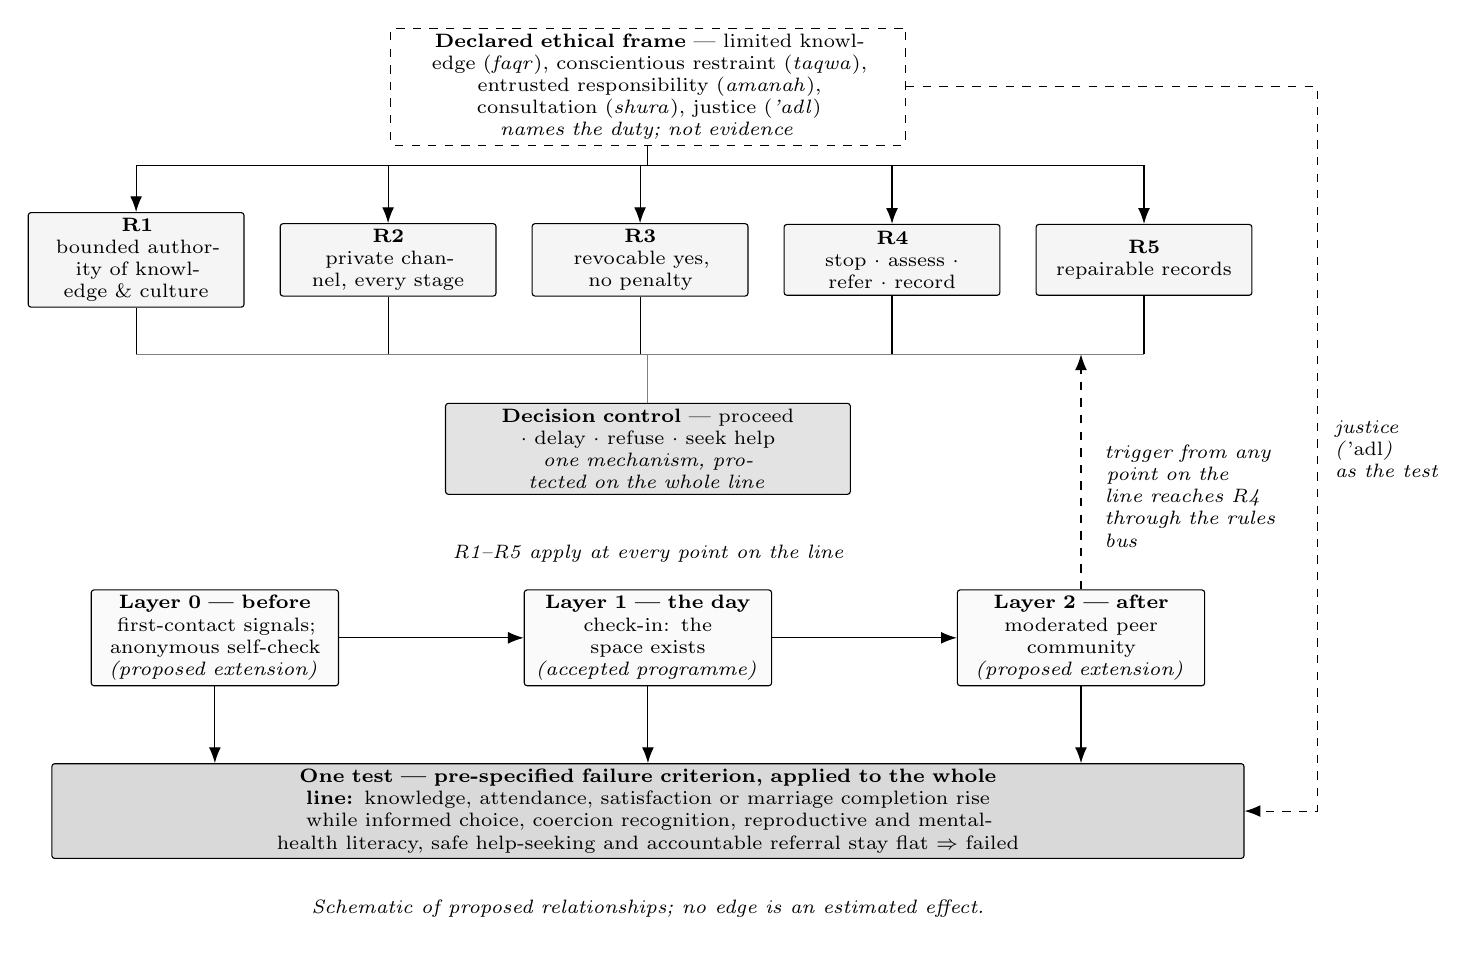
\begin{tikzpicture}[x=1mm,y=1mm,>={Latex[length=2mm]},
  box/.style={draw,rounded corners=1pt,fill=gray!8,align=center,font=\scriptsize,inner sep=2pt,minimum height=9mm},
  rule/.style={box,text width=26mm},
  layer/.style={box,text width=30mm,fill=gray!4},
  mech/.style={box,text width=50mm,fill=gray!22,minimum height=10mm},
  ethic/.style={box,text width=64mm,dashed,fill=white},
  test/.style={box,text width=150mm,fill=gray!30,minimum height=11mm},
  lab/.style={font=\scriptsize\itshape,align=left}]
\node[ethic] (E) at (85,100) {\textbf{Declared ethical frame} — limited knowledge (\emph{faqr}), conscientious restraint (\emph{taqwa}),\\ entrusted responsibility (\emph{amanah}), consultation (\emph{shura}), justice (\emph{\textquoteright adl})\\ \emph{names the duty; not evidence}};
\node[rule] (R1) at (20,78) {\textbf{R1}\\bounded authority of knowledge \& culture};
\node[rule] (R2) at (52,78) {\textbf{R2}\\private channel, every stage};
\node[rule] (R3) at (84,78) {\textbf{R3}\\revocable yes, no penalty};
\node[rule] (R4) at (116,78) {\textbf{R4}\\stop $\cdot$ assess $\cdot$ refer $\cdot$ record};
\node[rule] (R5) at (148,78) {\textbf{R5}\\repairable records};
\node[mech] (M) at (85,54) {\textbf{Decision control} — proceed $\cdot$ delay $\cdot$ refuse $\cdot$ seek help\\ \emph{one mechanism, protected on the whole line}};
\node[layer] (L0) at (30,30) {\textbf{Layer 0 — before}\\first-contact signals; anonymous self-check\\ \emph{(proposed extension)}};
\node[layer] (L1) at (85,30) {\textbf{Layer 1 — the day}\\check-in: the space exists\\ \emph{(accepted programme)}};
\node[layer] (L2) at (140,30) {\textbf{Layer 2 — after}\\moderated peer community\\ \emph{(proposed extension)}};
\node[test] (T) at (85,8) {\textbf{One test — pre-specified failure criterion, applied to the whole line:} knowledge, attendance, satisfaction or marriage completion rise\\ while informed choice, coercion recognition, reproductive and mental-health literacy, safe help-seeking and accountable referral stay flat $\Rightarrow$ failed};
\draw (E.south) -- (85,90);
\draw (20,90) -- (148,90);
\foreach \r in {R1,R2,R3,R4,R5} \draw[->] (\r.north |- 0,90) -- (\r.north);
\foreach \r in {R1,R2,R3,R4,R5} \draw (\r.south) -- (\r.south |- 0,66);
\draw[gray] (20,66) -- (148,66);
\draw[gray] (85,66) -- (M.north);
\draw[->] (L0.east) -- (L1.west); \draw[->] (L1.east) -- (L2.west);
\node[lab,anchor=north] at (85,43) {R1--R5 apply at every point on the line};
\foreach \l in {L0,L1,L2} \draw[->] (\l.south) -- (\l.south |- T.north);
\draw[->,dashed] (L2.north) -- (140,66);
\node[lab,anchor=west,text width=23mm] at (142,48) {trigger from any point on the line reaches R4 through the rules bus};
\draw[->,dashed] (E.east) -- (170,100) -- (170,8) -- (T.east);
\node[lab,anchor=west] at (171,54) {justice\\ (\emph{\textquoteright adl})\\ as the test};
\node[lab,anchor=north,font=\scriptsize\itshape] at (85,-2) {Schematic of proposed relationships; no edge is an estimated effect.};
\end{tikzpicture}}
\caption{Programme-theory diagram of \tphe, not a measured causal graph: no arrow represents an estimated effect. The declared ethical frame names the duty behind each rule; it is not evidence. Five pre-specified rules (R1--R5) are proposed to protect the single proposed mechanism, decision control; they apply at every point on one continuous timeline, of which only Layer~1 (the day) belongs to the accepted programme --- Layers~0 and~2 are extensions proposed for co-design. One pre-specified test is applied to the whole line; a trigger from any point can invoke R4 (stop--assess--refer--record) directly, and justice (\emph{\textquoteright adl}) is the standard the failure criterion itself is tested against.}
\label{fig:framework}
\end{figure}

\textbf{Definition and scope.} Trustworthy Premarital Health Education (\tphe) is a proposed governance architecture for premarital education. It is designed to increase each participant's control over marriage-related health decisions, through five rules, a stop--assess--refer--record pathway, repairable documentation, and prospectively testable outcomes (Figure~\ref{fig:framework}). \emph{Trustworthy} names a condition the programme must earn through observable practice. \emph{Premarital} names the transition point, not one legal or religious form. \emph{Health education} spans physical, psychological, sexual and reproductive, relational, legal-protection, and help-seeking literacy, without turning educators into clinicians, lawyers, investigators, or religious adjudicators. \emph{Infrastructure} means repeatable roles, boundaries, records, referral relationships, training, and accountability. \tphe{} sits upstream of a marriage; where it encounters existing violence or coercion, its role changes to identification and safe routing to competent services, not providing them directly. \tphe{} is \emph{not}: a diagnostic instrument; a substitute for clinical, legal, or survivor-advocacy services; couple therapy; a promise to prevent violence; a requirement that any participant proceed; a universal religious ruling; evidence that any organisation's programme works; or an autonomous AI counselling system.

\textbf{Mechanism and the six-to-five mapping.} \tphe{} rests on one mechanism: it is designed to increase each participant's control over whether to proceed with, delay, or refuse marriage, and over when and how to seek help. Six safeguards are proposed to protect decision control: epistemic humility, cultural intelligibility, affected-person visibility, dignity and consent, bounded authority and referral, and repairability. These are operationalised below as five auditable rules, R1--R5 (Table~\ref{tab:rules}). Epistemic humility and cultural intelligibility answer the same audit question --- whose authority is this claim carrying, and where does that authority end --- so they are implemented together as R1 (bounded authority of knowledge and culture). Affected-person visibility maps to R2; dignity and consent to R3; bounded authority and referral splits across R1 and R4; repairability maps to R5. Every safeguard survives this operationalisation; the change from six to five is a regrouping of duties into auditable rules, not a retraction of any safeguard.

\begin{table}[t]
\centering\footnotesize
\caption{The five rules (R1--R5): duty, one observable trace, one falsifier. Programme theory; none of these traces has yet been measured against an outcome.}
\label{tab:rules}
\begin{tabularx}{\textwidth}{@{}p{0.7cm}YYY@{}}
\toprule
& \textbf{Duty} & \textbf{Trace} & \textbf{Falsifier}\\
\midrule
R1 & Bounded authority of knowledge/culture: state what is known, uncertain, or needs qualified advice; culture or religion never closes a safety or consent question. & Uncertainty and role boundaries stated; out-of-scope referral. & A cultural/religious claim used to end, not refer, a safety or consent question.\\
R2 & A private channel for every person, every stage, the partner cannot see or control; professional interpreter, never a family member. & Routinely offered private slot; uptake logged without content. & A wanted private slot was denied, or family interpreted a safety-relevant exchange.\\
R3 & Revocable yes: pause, delay, refusal, or non-completion is normal, without penalty, at any point. & Pause/delay/refusal recorded without penalty. & A participant who paused or refused was excluded or pressured to reverse.\\
R4 & Stop--assess--refer--record: a trigger stops joint work, moves to private assessment by a competence-bounded assessor, refers to a qualified service (e.g.\ the OSCC), and records the sequence; joint work never resumes where coercive control is confirmed.\textsuperscript{a,b} & Time from trigger to qualified assessment; referral offered, connected, recorded. & Joint work continued/resumed without documented safe assessment, or a case closed by facilitator judgement without safeguarding-lead sign-off.\\
R5 & Repairable records: every entry has a named owner, a review date, and is corrected when new information arrives. & Review completed on schedule with dated correction. & A record never reviewed, or a correction overwriting the original entry.\\
\bottomrule
\end{tabularx}
\smallskip

\noindent\footnotesize\textsuperscript{a}If no qualified assessor is reached within a pre-specified interval, or assessment is inconclusive, the default is continued stop, escalated to a named safeguarding lead. \textsuperscript{b}Proposed extension: the assessor should also have no stake in the wedding and no compromising prior relationship with either participant (analogy evidence only \cite{ref158,ref162}).
\end{table}
\FloatBarrier

\textbf{Three layers on a continuous line.} The programme theory does not treat the classroom day alone as the intervention. It treats the whole trajectory, from first contact through the day of check-in to whatever follows, as one governed line, on which the mechanism, five rules, and one failure criterion apply throughout (Figure~\ref{fig:framework}). \emph{Layer~0 (proposed extension, not part of the accepted programme)} is signals from first contact: course material can name what fear, control, or unsafe participation look like, and an anonymous scored self-check lets a person see their own result. The nearest evidence family is decision-aid research, not a validated self-check for this population: a Cochrane review of 209 decision-aid trials found consistent gains in knowledge and values-congruent choice \cite{ref14}, while the closest content-matched tool for women experiencing abuse, I-DECIDE, found no improvement in self-efficacy at 6 or 12 months in an RCT \cite{ref120}; that null result is reported, not set aside. \emph{Layer~1 (the accepted programme)} is the day as check-in: a participant verifies in person that declared protections are in place, including a private slot, a professional interpreter, and an assessor with no stake in the wedding; attendance shows the space exists, not that the programme changed anyone's decisions or safety. \emph{Layer~2 (proposed extension)} is a moderated peer community after the course: moderation quality is repeatedly identified in realist syntheses as the factor determining whether such a space helps or harms \cite{ref140,ref144}, and technology-facilitated-abuse research documents how an unmoderated digital channel can itself become a vector for coercive control \cite{ref149,ref150}; neither literature was generated on a Muslim or Thai premarital population, and the pairing is by analogy.

\textbf{What would show it failed.} The programme theory has one pre-specified failure criterion. It applies to the mechanism, the rules, and every layer together. \tphe{} fails if it raises knowledge scores, attendance, satisfaction, or marriage completion while leaving informed choice, recognition of coercion, reproductive and mental-health literacy, safe help-seeking, and accountable referral unchanged.

\textbf{Safeguarding specification.} If danger appears imminent, the routine R4 sequence is suspended: immediate safety planning and contact with emergency services or the OSCC emergency line take precedence over scheduling confidential assessment, and facilitators are never the final decision-maker for either pathway. If a qualified assessor cannot be reached in time, or assessment is inconclusive, the default is continued stop, escalated to a named safeguarding lead independent of routine facilitation duty. Administrative and safeguarding records are kept separate, with restricted access, a defined retention period, and a default to non-disclosure for third-party requests absent a legal requirement, complying with Thailand's Personal Data Protection Act B.E.~2562 (PDPA). The full operational checklist (before, during, triggered, and after delivery) is given in the online supplementary material (Appendix S4). \textbf{Minors boundary.} \tphe{}'s safeguards assume adult participants able to consent in their own right. Where a participant is, or may be, a minor, duty-of-care and mandatory-reporting obligations take precedence over the framework's consent-based rules (R2, R3); this interface is not yet specified, and specifying it is a named prerequisite for Phase~1 (see Research and development pathway).

\textbf{Testable propositions.} Table~\ref{tab:rules} converts the framework into a research agenda; it is designed to produce disconfirming evidence, not a set of findings. Seven propositions are pre-specified (full statements, competing explanations, and falsifying evidence: online supplementary material, Appendix~S3):
\begin{itemize}
\item P1: whether a governance layer improves decision control beyond content-only education.
\item P2: whether a routine private channel makes materially relevant concerns more visible.
\item P3: whether R1's cultural-intelligibility component improves comprehension and trust only when culture or religion cannot override consent or safety.
\item P4: whether a stop rule prevents routine joint education from worsening risk when fear or coercion appears.
\item P5: whether referral quality depends on timeliness, accessibility, and follow-through, not offer alone.
\item P6: whether conventional programme success can coexist with \tphe{} failure.
\item P7: whether repairable records (R5) are necessary because relevant information emerges over time.
\end{itemize}
Each proposition is paired with a competing explanation and with a falsifier\footnote{A falsifier is the specific observation that, if seen, would show the rule or proposition failed.} --- the evidence that would weaken or falsify it --- so a null or contrary result changes the framework rather than being absorbed by it.

\textbf{Research and development pathway.} Five phases are planned, using the MRC framework's development-to-evaluation logic \cite{ref52}. Phase~0: framework clarification and evidence mapping, including legal and data-governance review. Phase~1: co-design and content validation with survivors and advocates, community members, and relevant professionals, chaired independently of ARAYA Nikah, with any survivor- or community-facing activity approved by an accredited Thai research-ethics committee first. Phase~2: a feasibility and safety pilot, testing whether \tphe{} can be delivered safely and consistently, not whether it reduces violence. Phase~3: prospective comparative evaluation, with decision control as the primary candidate outcome; the failure criterion and primary outcome set will be registered publicly (e.g., the Thai Clinical Trials Registry, TCTR) before data collection begins. Phase~4: independent replication outside ARAYA, in different legal, service, religious, and cultural settings. Minors are out of scope until the minors boundary named under Safeguarding specification is completed and approved.

\section{Discussion}

\subsection{Principal findings}
\tphe{} shifts the organising question of premarital education from content delivery to the governance of choice. Values such as respect, consent, culture, and referral become trustworthy only when translated into roles, trigger criteria, private channels, competence boundaries, records, review points, and measurable outcomes.

\subsection{Novelty}
\tphe{} is not proposed into an empty field. Table~\ref{tab:novelty} places it alongside adjacent bodies of practice and evidence, stating only what each is documented to do, measure, and not do, and what \tphe{} adds on top of it; the comparison is not a claim that \tphe{} outperforms any row, and no effectiveness evidence exists for \tphe{} itself. This comparison is drawn from published and indexed descriptions only; curricula and manuals were not obtained, so comparable safeguards may exist undocumented in any row.

\begin{table}[t]
\centering\footnotesize
\caption{What existing frameworks and programmes do, measure, and do not do, against what \tphe{} makes explicit and auditable. Descriptive only; several rows are not examined here at manual/curriculum level. No effectiveness comparison is implied.}
\label{tab:novelty}
\begin{tabularx}{\textwidth}{@{}p{2.5cm}YY@{}}
\toprule
& \textbf{Documented scope and gap} & \textbf{What \tphe{} makes explicit and auditable}\\
\midrule
WHO RESPECT & Names relationship-skills strengthening as one of seven population-level prevention strategies, but only 6/178 reviews updating it targeted that strategy \cite{who_respect,ref30}. & A governance layer with a named mechanism and stop rule, inside RESPECT's relationship-skills strategy, at the marriage transition specifically.\\
Thai premarital course, Health Region~12 & Government health-region delivery in Thailand's southern provinces; no outcome study identified in PubMed as of 2026-09; the course manual was not examined (search limited to PubMed). & A published, auditable rule set (R1--R5) and failure criterion any programme can be checked against.\\
Malaysian Kursus Pra-Perkahwinan Islam (Islamic Pre-Marriage Course) & Reportedly administratively linked to marriage registration, not independently verified here; analysed only through a moral-education lens at one centre \cite{charoenwong2025} (non-PubMed, context only); not shown to measure decision control. & A decision-control mechanism and stop rule layered onto mandatory delivery, not assumed present in it.\\
Relationship\slash marriage education (MRE, PREP) & Structured curricula evaluated in cumulative meta-analyses; effects small ($d\approx0.03$--$0.45$), higher-conflict couples fared worse in one 8-year RCT \cite{ref6,ref7,ref9,fawcett2010}. & A stop rule withholding joint communication/conflict training precisely where coercive control is suspected.\\
IPV screening in health settings & Increases identification (OR~2.95) but no shown effect on referral or re-exposure \cite{ref38,ref39}. & Referral counted at connection, not offer, plus a record reviewed and corrected rather than closed at first entry.\\
Digital safety decision aids (I-DECIDE) & Scored self-directed tools; the largest RCT found no self-efficacy gain at 6 or 12 months \cite{ref120}; not built for the premarital transition. & An anonymous self-check as one entry point on a line that also includes an in-person check-in and a named stop rule.\\
\bottomrule
\end{tabularx}
\end{table}
\FloatBarrier

Read across the rows, \tphe{}'s claimed novelty is not a new curriculum topic; every topic already exists somewhere in the comparison. The novelty is a governance layer placed around premarital education, with decision control named as the mechanism, rather than knowledge gain, attendance, satisfaction, or completion. Four design choices follow directly from documented gaps. A private channel at every stage answers the finding that screening increases identification without a shown effect on referral \cite{ref38,ref39}. The stop rule follows from the couples-therapy literature's own caution: the only systematic review of conjoint IPV treatment, after screening 1{,}733 citations to 6 eligible studies, called it viable only in select situations \cite{ref45}, and clinical literature treats distinguishing situational couple violence from coercive controlling violence as a prerequisite for joint work \cite{ref46,ref47}. Counting referral at connection, not offer, follows from an emergency-department programme in which most screened patients could not recall receiving a resource guide \cite{ref173}. Repairable records and the failure criterion follow from a knowledge-to-behaviour gap documented twice: premarital screening and thalassaemia education raise knowledge without matching uptake \cite{ref12,ref13}, and decision-aid research shows values-congruent choice can improve while self-efficacy did not \cite{ref14,ref120}.

\subsection{Comparison with the wider evidence base}
\tphe{} is compared here against the literature it draws on and is answerable to, not against a systematic review's full search strategy. Every citation offers adjacent, analogous, or precedent evidence for a construct \tphe{} uses, never evidence that \tphe{} itself works. The full evidence review, organised by proposition, is reported in the online supplementary material (Appendix S1). Four patterns recur there and are load-bearing for the design. First, knowledge does not reliably convert into protective behaviour at existing premarital contact points: thalassaemia education raises knowledge ($p<0.001$) without reliably raising screening uptake \cite{ref13}, and premarital sickle-cell-trait screening uptake across Africa remains under half of eligible couples (47.8\%) \cite{ref12}. Second, identification does not reliably convert into referral: a Cochrane review of 13 RCTs found screening increased identification (OR~2.95) with no shown effect on referral (OR~2.24) or re-exposure at 3--18 months \cite{ref38}, and the 2025 US Preventive Services Task Force (USPSTF) evidence report found no significant reduction in IPV over 3--18 months in 3 comparative RCTs \cite{ref39,ref40}. Third, cultural-competence training repeatedly raises provider-level knowledge or attitudes without a corresponding patient-outcome gain: a Cochrane review of 5 RCTs \cite{ref55}, a narrower review \cite{ref56}, and cross-country Indigenous cultural-safety training \cite{ref57} all found this pattern --- the gap R1 is built to answer, not assume solved. Fourth, recognition and behaviour dissociate: a 1-year cluster RCT of a coach-delivered dating-violence prevention programme found perpetration fell, but recognition of abusive behaviours did not change (95\% CI $-0.15$ to $0.09$) \cite{ref190}, exactly the separation \tphe{}'s failure criterion is built to catch. The stop rule's own evidence base is small and explicitly cautious: the only systematic review of couples therapy as IPV treatment found 6 eligible studies, judging conjoint treatment ``viable in select situations'' \cite{ref45}. Direct Thai evidence remains sparse: a four-region national survey found roughly 15\% lifetime psychological, physical, or sexual IPV among married or cohabiting women \cite{ref72}. No study identified evaluates a premarital-education programme, of any design, with a Thai Muslim or Thai intercultural population.

\subsection{Declared ethical frame}
\emph{Transliteration note: Arabic terms are given in plain italic script (e.g., \emph{faqr}, \emph{\textquoteright adl}) throughout this paper; the framework itself is operable without this vocabulary, which is supplied here as provenance, not as a requirement for adoption by non-Muslim programmes.}

The framework does not treat culture as a barrier to be removed. Its epistemic-humility safeguard rests on a working sequence of five terms, in the order Table~\ref{tab:ethic} uses:
\begin{itemize}
\item \emph{Faqr} (limited knowledge): awareness of our own incompleteness and dependence on God.
\item \emph{Taqwa} (conscientious restraint): God-conscious restraint over one's knowledge, speech, judgement, and use of power.
\item \emph{Amanah} (entrusted responsibility): authority and knowledge are an entrusted responsibility, rendered to those to whom it belongs.
\item \emph{Shura} (consultation): the method of acting when limits are reached.
\item \emph{\textquoteright Adl} (justice): the test --- not whether the person holding authority meant well, but whether the affected person retains dignity, rights, voice, and a real route to correction.
\end{itemize}
Table~\ref{tab:ethic} pairs each term with the rule it governs and an evidence tier; where a pairing is Open, the rule is supported only by its own falsifier and observable trace (Table~\ref{tab:rules}), not by external evidence for the ethical term. This is compatible with cultural humility in health education \cite{ref58}. Tier-one Islamic bioethics literature gives this ethical frame real companions in the medical literature, without becoming evidence that the frame, or \tphe{}, works \cite{ref225,ref228}. Faith-integrated delivery can carry a measurable clinical effect: a cluster-randomised mosque-based diabetes-prevention trial reduced 12-month type~2 diabetes incidence from 17.1\% to 9.8\% (adjusted hazard ratio 0.75, 95\% CI 0.60--0.95) \cite{ref231}. No indexed premarital guideline from the Federation of Islamic Medical Associations (FIMA) or the Islamic Medical Association of North America (IMANA), and no Thai Muslim premarital trial, exists in this record.

Culture-and-health scholarship more broadly supplies theoretical warrant, not efficacy evidence, for treating culture as a determinant the safeguards must hold rather than resolve; a meta-analysis of 67 randomised trials of culturally adapted psychological interventions for people of Chinese descent found a medium overall effect but no significant difference between adaptation types \cite{ref89} --- evidence against assuming any one adaptation strategy superior, not against cultural adaptation itself. Two structured-social-support trials outside the marriage-transition setting offer an analogy, not evidence, for the mechanism the safeguards are built around \cite{ref90,ref91}.

\begin{table}[t]
\centering\footnotesize
\caption{The declared ethical frame: term, governed rule, evidence category, and evidence tier. The term names a duty; the evidence category speaks to the construct, not the term. External-evidence and analogy citations are from adjacent, non-Thai, non-Muslim, non-premarital populations unless stated otherwise.}
\label{tab:ethic}
\begin{tabularx}{\textwidth}{@{}p{1.3cm}p{1.4cm}YY@{}}
\toprule
\textbf{Term} & \textbf{Governs} & \textbf{Evidence category} & \textbf{Tier}\\
\midrule
Faqr & R1 & Intellectual/relational humility literature (adjacent populations). & External (analogy); no Muslim/Thai samples.\\
Taqwa & R1, R4 & Self-regulation and provider-boundary literature. & Open: no pairing identified for this population.\\
Amanah & R2, R3, R5 & Consent, autonomy, accountability literature. & Open: no pairing identified for this population.\\
Shura & R4 & Independent-advocate/dual-relationship literature \cite{ref159,ref163}. & Analogy: transplant-advocate and dual-relationship ethics, not domain-matched.\\
'Adl & Failure criterion & Outcome-domain and safeguarding literature the criterion is built from. & Practitioner-derived; authored for this paper.\\
\bottomrule
\end{tabularx}
\end{table}
\FloatBarrier

\subsection{Institutional position}
Why does a social enterprise convene this synthesis? The answer is a declared position, not an evidentiary claim: it rests on process, not authority. ARAYA Nikah sits with a couple across the weeks before a wedding, controls the sequence in which content, documentation, and referral are offered, and observes where consent, authority, and help-seeking are organised. It is registered under Thailand's Social Enterprise Promotion Act B.E.~2562, which binds it to a declared social objective and limits profit distribution; because continuation does not depend on completing marriages, it can treat marriage completion as irrelevant to success. This position carries no authority of its own: its legitimacy is borrowed, not earned, and stands until survivors, advocates, religious and community leaders, and independent reviewers say whether these procedures hold up.

\subsection{Strengths and limitations}
Strengths: the programme theory is stated with a pre-specified failure criterion, named outcome domains, and testable propositions with falsifiers, before any effectiveness testing; the claim ceiling is explicit; the conflict of interest is disclosed. Limitations: (1)~derived from one founder-led organisation; (2)~not a formal qualitative study --- no systematic sampling, independent coding, saturation, or participant validation; (3)~no effectiveness or safety testing, so the mechanism, safeguards, measures, and pathway may prove incomplete, burdensome, or harmful; (4)~grounded in Muslim and intercultural couples in Thailand, not representative of all Muslim communities, Thai settings, or non-Muslim contexts; (5)~identifies a governance problem without establishing that existing programmes lack comparable safeguards; (6)~decision control is not a validated measure and may overlap with autonomy, self-efficacy, informed choice, safety, and service access; (7)~referral capacity is context-dependent; (8)~founder authorship creates conflict of interest, so independent co-design, external review, and replication are necessary; (9)~AI was not used for counselling, safety decisions, or classifying violence or coercion in this work (Declarations gives the AI-use boundary in full).

\subsection{Implications for practice, policy, and research}
Without a failure criterion, programmes can absorb safeguarding language while keeping continuation-oriented incentives; infrastructure should be judged by what it enables under pressure, not ideal conditions. \tphe{} originated in a Muslim-led Thai practice environment but addresses a general problem; transferability is empirical, assessed using the MRC's own ADAPT\footnote{ADAPT: a named MRC guidance package for adapting evidence-based interventions to new contexts, not an acronym expanded by its source.} guidance \cite{ref53}. Adaptation may change language, examples, religious sources, legal procedures, service partners, and settings, but must preserve these invariants:
\begin{itemize}
\item the participant, not marriage completion, is the unit of protection;
\item usable decision control is the mechanism;
\item each person has a safe private route;
\item culture and religion do not override consent or safety;
\item educator authority is bounded;
\item fear or coercive control changes the course of education;
\item qualified referral takes priority beyond competence;
\item decisions and records can be reviewed and corrected.
\end{itemize}

\subsection{How to test it with us}
This framework is offered at the point where practice-derived synthesis must stop and shared testing must begin. ARAYA Nikah does not propose to validate \tphe{} alone, and does not claim the authority to decide what ``trustworthy'' means for communities it does not represent. It can offer what this paper has made explicit and auditable: its governance and safeguarding procedures, its stop--assess--refer--record pathway, its practice context of 600+ participants (demand for this work, not evidence that it succeeds), and a pre-specified failure criterion it is willing to be judged against. Co-design needs partners this paper cannot substitute for: survivors and advocates; Health Region~12 and its existing premarital services; provincial Islamic committees; and referral services, including One-Stop Crisis Centres. Governance commitments for a first co-design phase (independent chair, decision authority, licensing, right to withdraw) are given in the online supplementary material (Appendix S4). Nothing proceeds to scale before a feasibility and safety pilot confirms \tphe{} can be delivered safely and consistently.

\section{Conclusion}
Premarital health education is a consequential decision environment. When it cannot protect the individual participant, stop unsafe joint work, refer beyond educator competence, or correct an earlier decision, it remains incomplete as public-health infrastructure. \tphe{} proposes one mechanism, decision control, operationalised as five rules (R1--R5) proposed to protect it, and a stop rule under which routine couple education yields to confidential assessment, survivor-centred support, and qualified referral. The framework is not yet validated; its value will depend on whether co-design and empirical testing show it improves usable choice and accountable routing without creating new harms. Premarital health education should be judged not by how many marriages it completes, but by how safely people can choose. That judgement is not the organisation's to make alone: clinical, public-health, religious, and community partners, referral services, survivors, and advocates are invited to co-design and test this framework together, under the failure criterion stated above, before any claim of effectiveness is made.

\FloatBarrier
\section*{Declarations}
\footnotesize
\textbf{Conflict of interest.} The author is the founder and programme developer of ARAYA Nikah Social Enterprise Co., Ltd., the organisation whose procedures informed this synthesis, and has a reputational and commercial interest in the programme described. This conflict is disclosed in every public version of the work. No grant or award funded this work. It is managed as follows: no ARAYA-affiliated person will chair the co-design phase or hold a veto in its steering group, and Phase~4 requires replication outside ARAYA (see The framework, Research and development pathway).\\
\textbf{Funding.} None.\\
\textbf{Ethics.} This conceptual paper involved no participant research, no participant data, and no identifiable information. Any co-design, cognitive interviewing, pilot data collection, or evaluation will undergo ethics review before it begins.\\
\textbf{Data availability.} No participant dataset was generated or analysed. The full manuscript source, extended evidence review, and scenario-simulation code and its declared parameters are available at \url{https://github.com/morrocwi/RE_T-PHE} and in the online supplementary material published alongside this article; further materials are available from the corresponding author on request.\\
\textbf{Use of AI.} AI tools assisted drafting and editing; the author verified all content and is accountable for it. No participant data are entered into any AI system; the anonymous self-check described in The framework (Layer~0), if used, is scored without AI.\\
\textbf{Author contributions.} YL conceived the framework, conducted the synthesis, and wrote the manuscript; there are no further contributors.\\
\textbf{Acknowledgements.} The author thanks the organisation's team for their support during the development of this work.\\
\textbf{Prior presentation.} A version of this work was presented at the TIMA/FIMA Scientific Convention 2026 (Thai Islamic Medical Association / Federation of Islamic Medical Associations); the accepted conference abstract is reproduced verbatim in the online supplementary material (Appendix S0), which remains the claim ceiling for this manuscript.\\
\textbf{Disclaimer.} This paper is a theoretical framework. It is not medical, legal, or religious advice, not a diagnostic instrument, and not a substitute for qualified clinical, legal, or survivor-support services. Laws governing health advice, safeguarding, data protection, and marriage vary by jurisdiction; institutional, educational, or public use requires legal and professional review.

\clearpage
\begin{thebibliography}{999}\footnotesize
\bibitem{who_vaw_2026} World Health Organization. Violence against women [fact sheet]. 2026. \url{https://www.who.int/news-room/fact-sheets/detail/violence-against-women}
\bibitem{ref1} GBD 2023 IPV and SVAC Collaborators. Disease burden attributable to intimate partner violence against females and sexual violence against children in 204 countries and territories, 1990-2023: a systematic analysis for the Global Burden of Disease Study 2023. Lancet (London, England). 2026. PMID: 41386261.
\bibitem{ref2} Sardinha L. Global, regional, and national prevalence estimates of physical or sexual, or both, intimate partner violence against women in 2018. Lancet (London, England). 2022. PMID: 35182472.
\bibitem{ref3} Kuswanto H. Prevalence of and factors associated with female child marriage in Indonesia. PLoS ONE. 2024. PMID: 38968277.
\bibitem{ref4} Rumble L. An empirical exploration of female child marriage determinants in Indonesia. BMC Public Health. 2018. PMID: 29587705.
\bibitem{ref5} Islam MK. Attitudes to and experiences of intimate partner violence among Rohingya women who married before eighteen years of age. Global Health Action. 2021. PMID: 34323166.
\bibitem{dwf2024} Department of Women's Affairs and Family Development, Thailand. Domestic violence [in Thai]. 2024. \url{https://www.dwf.go.th/contents/71825} (accessed 2026-09-02)
\bibitem{ref6} Hawkins AJ. Does marriage and relationship education work? A meta-analytic study. Journal of Consulting and Clinical Psychology. 2008. PMID: 18837590.
\bibitem{ref7} Hawkins AJ. How effective are ACF-funded couple relationship education programs? A meta-analytic study. Family Process. 2022. PMID: 35040124.
\bibitem{ref8} Karantzas Gery C. Do relationship education programs reduce relationship aggression? A meta-analytic study. Clinical Psychology Review. 2023. PMID: 37499317.
\bibitem{ref9} Markman HJ. A randomized clinical trial of the effectiveness of premarital intervention: moderators of divorce outcomes. Journal of Family Psychology. 2013. PMID: 23421844.
\bibitem{ref10} Williamson HC. Risk moderates the outcome of relationship education: a randomized controlled trial. Journal of Consulting and Clinical Psychology. 2015. PMID: 25664643.
\bibitem{ref11} Benedetto Chiara. FIGO Preconception Checklist: Preconception care for mother and baby. International Journal of Gynaecology and Obstetrics. 2024. PMID: 38426290.
\bibitem{ref12} Dilli Priscilla Peter. Update on the practice of premarital screening for sickle cell traits in Africa: a systematic review and meta-analysis. BMC Public Health. 2024. PMID: 38822327.
\bibitem{ref13} Anwar. Characteristics and Effectiveness of Premarital Thalassaemia Educational Interventions Worldwide: A scoping review. Sultan Qaboos University Medical Journal. 2025. PMCID: PMC12445309; not PubMed-indexed.
\bibitem{ref14} Stacey Dawn. Decision aids for people facing health treatment or screening decisions. Cochrane Database of Systematic Reviews. 2024. PMID: 38284415.
\bibitem{ref16} Upadhyay Ushma D. Development and validation of a reproductive autonomy scale. Studies in Family Planning. 2014. PMID: 24615573.
\bibitem{ref17} McCauley Heather L. Psychometric properties and refinement of the Reproductive Coercion Scale. Contraception. 2017. PMID: 27639927.
\bibitem{ref18} Upadhyay Ushma D. Development and Validation of the Sexual and Reproductive Empowerment Scale for Adolescents and Young Adults. The Journal of Adolescent Health. 2021. PMID: 32690468.
\bibitem{ref19} Dagher Myriam. Adaptation and psychometric assessment of a sexual and reproductive empowerment scale in Arabic among refugee and non-refugee adolescent girls. BMC Medical Research Methodology. 2024. PMID: 39266993.
\bibitem{ref20} Alomair N. Factors influencing sexual and reproductive health of Muslim women: a systematic review. Reproductive Health. 2020. PMID: 32138744.
\bibitem{ref52} Skivington K. A new framework for developing and evaluating complex interventions: update of Medical Research Council guidance. BMJ. 2021. PMID: 34593508.
\bibitem{ref53} Moore G. Adapting interventions to new contexts-the ADAPT guidance. BMJ. 2021. PMID: 34344699.
\bibitem{ref54} Moore GF. Process evaluation of complex interventions: Medical Research Council guidance. BMJ. 2015. PMID: 25791983.
\bibitem{ref30} Ullman C. Interventions to prevent violence against women and girls globally: a global systematic review of reviews to update the RESPECT women framework. BMJ Public Health. 2025. PMID: 40017928.
\bibitem{ref38} O'Doherty L. Screening women for intimate partner violence in healthcare settings. Cochrane Database of Systematic Reviews. 2015. PMID: 26200817.
\bibitem{ref39} Feltner Cynthia. Screening for Intimate Partner Violence and for Caregiver Abuse of Older or Vulnerable Adults: An Evidence Report and Systematic Review for the US Preventive Services Task Force. JAMA. 2025. PMID: 40553460.
\bibitem{ref40} US Preventive Services Task Force. Screening for Intimate Partner Violence and Caregiver Abuse of Older or Vulnerable Adults: US Preventive Services Task Force Recommendation Statement. JAMA. 2025. PMID: 40553450.
\bibitem{ref45} Karakurt. Couples Therapy for Intimate Partner Violence: A Systematic Review and Meta-Analysis. Journal of marital and family therapy. 2016. PMID: 27377617.
\bibitem{ref46} McCollum. Couples treatment for interpersonal violence: a review of outcome research literature and current clinical practices. Violence and victims. 2008. PMID: 18624089.
\bibitem{ref47} Schneider. From scared to repaired: using an attachment-based perspective to understand situational couple violence. Journal of marital and family therapy. 2014. PMID: 25039387.
\bibitem{ref55} Horvat L. Cultural competence education for health professionals. Cochrane Database of Systematic Reviews. 2014. PMID: 24793445.
\bibitem{ref56} Vella Elizabeth. Does cultural competence training for health professionals impact culturally and linguistically diverse patient outcomes? A systematic review of the literature. Nurse Education Today. 2022. PMID: 35964378.
\bibitem{ref57} Hardy Billie-Jo. Systematic review of Indigenous cultural safety training interventions for healthcare professionals in Australia, Canada, New Zealand and the United States. BMJ Open. 2023. PMID: 37793931.
\bibitem{ref58} Tervalon M. Cultural humility versus cultural competence: a critical distinction in defining physician training outcomes in multicultural education. Journal of Health Care for the Poor and Underserved. 1998. PMID: 10073197.
\bibitem{ref72} Chuemchit Montakarn. Prevalence of Intimate Partner Violence in Thailand. Journal of Family Violence. 2018. PMID: 29904232.
\bibitem{ref120} Hegarty K et al. An online healthy relationship tool and safety decision aid for women experiencing intimate partner violence (I-DECIDE): a randomised controlled trial. The Lancet Public Health. 2019; PMID: 31155223.
\bibitem{ref89} Li S. Efficacy of culturally adapted interventions for common mental disorders in people of Chinese descent: a systematic review and meta-analysis. Lancet Psychiatry. 2023. PMID: 37208113.
\bibitem{ref90} Axinn WG. Community-Level Social Support Infrastructure and Adult Onset of Major Depressive Disorder in a South Asian Postconflict Setting. JAMA Psychiatry. 2022. PMID: 35080609.
\bibitem{ref91} Watt RG. Effectiveness and cost-effectiveness of a parenting programme to improve family wellbeing in England (TOGETHER): a multicentre, single-blind, randomised controlled trial. Lancet Public Health. 2026. PMID: 41887826.
\bibitem{ref190} Miller E et al. One-year follow-up of a coach-delivered dating violence prevention program: a cluster randomized controlled trial. American journal of preventive medicine. 2013; PMID: 23790995.
\bibitem{ref140} Marshall P et al. Understanding the Impacts of Online Mental Health Peer Support Forums: Realist Synthesis. JMIR Mental Health. 2024; PMID: 38722680.
\bibitem{ref144} Deng D et al. The Role of Moderators in Facilitating and Encouraging Peer-to-Peer Support in an Online Mental Health Community: A Qualitative Exploratory Study. Journal of Technology in Behavioral Science. 2023; PMID: 36810998.
\bibitem{ref149} Rogers MM et al. Technology-Facilitated Abuse in Intimate Relationships: A Scoping Review. Trauma, Violence \& Abuse. 2023; PMID: 35537445.
\bibitem{ref150} Henry N et al. Technology-Facilitated Domestic and Sexual Violence: A Review. Violence Against Women. 2020; PMID: 32998673.
\bibitem{ref158} Robbins KC et al. The Independent Living Donor Advocate: An Essential Role for Living Kidney Donation. Nephrology Nursing Journal. 2014; PMID: 26287054.
\bibitem{ref159} Rudow DL et al. The Psychosocial and Independent Living Donor Advocate Evaluation and Post-surgery Care of Living Donors. Journal of Clinical Psychology in Medical Settings. 2015; PMID: 26293351.
\bibitem{ref162} Pope KS et al. Dual relationships in psychotherapy. Ethics \& Behavior. 1991; PMID: 11649348.
\bibitem{ref163} Scopelliti J et al. Dual relationships in mental health practice: issues for clinicians in rural settings. Australian and New Zealand Journal of Psychiatry. 2004; PMID: 15555031.
\bibitem{ref173} Loo S et al. Evaluating a social risk screening and referral program in an urban safety-net hospital emergency department. Journal of the American College of Emergency Physicians Open. 2023; PMID: 36704207.
\bibitem{ref225} Mustafa Y et al. Islam and the four principles of medical ethics. Journal of Medical Ethics. 2014; PMID: 23975951.
\bibitem{ref228} Padela AI et al. Islamic medical ethics: a primer. Bioethics. 2007; PMID: 17845488.
\bibitem{ref231} Bhowmik B et al. Faith-Based Lifestyle Intervention for Diabetes Prevention Among Adults in Bangladesh: A Cluster Randomized Clinical Trial. JAMA Network Open. 2025; PMID: 41114978.
\bibitem{who_respect} World Health Organization. RESPECT women: preventing violence against women. 2nd ed. Geneva: WHO; 2025. ISBN 9789240117020. Not PubMed-indexed.
\bibitem{fawcett2010} [Not PubMed-indexed; cited for transparency only.] Fawcett EB, Hawkins AJ, Blanchard VL, Carroll JS. Do premarital education programs really work? A meta-analytic study. \emph{Fam Relat}. 2010;59(3):232--239. \url{https://doi.org/10.1111/j.1741-3729.2010.00598.x}
\bibitem{charoenwong2025} Charoenwong W. Islamic premarital education in Malaysia through the lens of moral education. \emph{Asia-Pacific Social Science Review}. 2025. (Volume and page numbers not yet assigned by the publisher at time of writing.)
\end{thebibliography}

\end{document}
